\begin{Example}[toxaemia0]{Toxaemic symptoms in pregnancy}
In \secref{sec:loglin-multiv}, we examine multivariate models
for two or more categorical responses.
\exref{ex:toxaemia} presents an analysis of data from
\citet{Brown-etal:83}
on the occurrence of two
signs of toxaemia (hypertension and protein urea)
among 13,384 expectant mothers in Bradford, England in their first pregnancy.
The mothers are classified by social class (1--5), and by the
number of cigarettes smoked per day (0, 1--19, or $20+$).

The models presented later describe how both the marginal distributions
of the responses, \emph{and} their association, vary with explanatory variables.
Here, we preview those data with a fourfold display focused on just
the association (odds ratio) between the two binary
response variables, Hypertension and Urea.


%% one figure
\begin{figure}[htb]
  \centering
  \includegraphics[width=\linewidth,clip]{ch3/fig/4ftox.eps}
  \caption[Fourfold display for toxaemia data]{Fourfold display for toxaemia data.  The level of mother's smoking increases from top to bottom;
  mother's social class increases from left to right}%
  \label{fig:4ftox}
\end{figure}

\figref{fig:4ftox} shows the fourfold displays for the 15 combinations
of mother's social class and smoking, with non-smokers in the top row,
and heaviest smokers in the bottom row.
We see that, with one exception (a cell with small total frequency),
the association between presence of hypertension and urea
is positive, and roughly of the same magnitude over the categories
of class, particularly for non- and moderate-smokers.
In \exref{ex:toxaemia} we plot the log odds ratio directly (\figref{fig:tox13}), as well as the log odds for prevalence
of these two symptoms.
\end{Example}
